\subsubsection{Caso d'uso UC8.1.3.5: Creazione domanda a ordinamento di immagini}
\label{UC8.1.3.5}
	\begin{figure}[h]
		\centering
			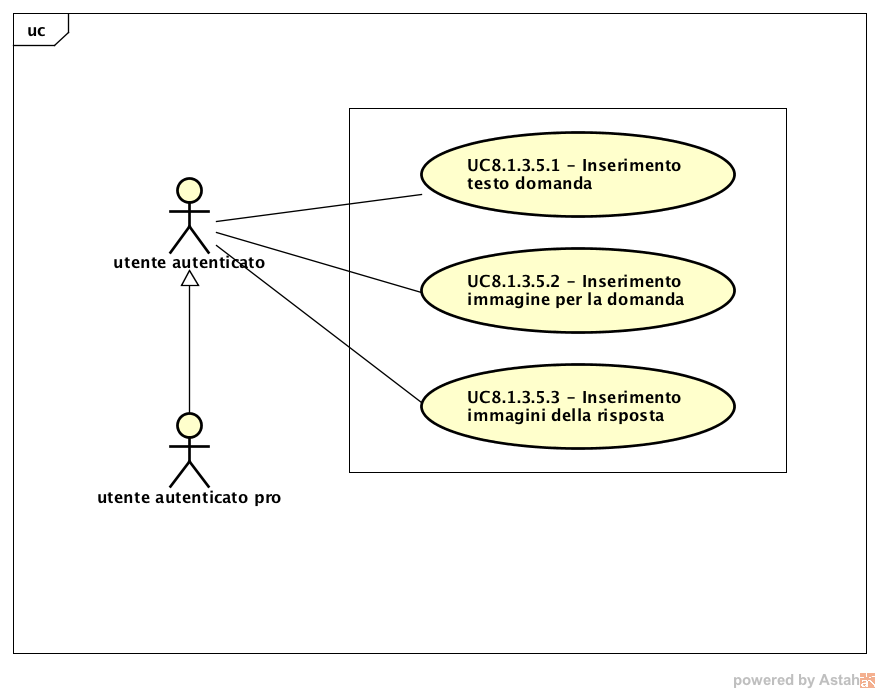
\includegraphics[scale=0.45,keepaspectratio]{UML/UC8_1_3_5.png}
		\caption{UC8.1.3.5: Creazione domanda a ordinamento di immagini}
	\end{figure}
	\FloatBarrier
\begin{itemize}
	\item\textbf{Attori}: utente autenticato, utente autenticato pro;
	\item\textbf{Descrizione}: l'attore può utilizzare la procedura guidata per la creazione di una domanda a ordinamento di immagini;
	\item\textbf{Precondizione}: l'attore ha selezionato la funzionalità di creazione di una domanda a ordinamento di immagini; 
	\item \textbf{Postcondizione}: l'attore ha creato una domanda a ordinamento di immagini;
	\item\textbf{Scenario principale}:
	\begin{itemize}
		\item L'attore può inserire il testo della domanda (UC8.1.3.5.1);
		\item L'attore può inserire un'immagine relativa al testo della domanda (UC8.1.3.5.2);
		\item L'attore può inserire le immagini della sequenza che costituirà la risposta (UC8.1.3.5.3).
	\end{itemize}
\end{itemize}

\subsubsection{Caso d'uso UC8.1.3.5.1: Inserimento testo della domanda}
\begin{itemize}
	\item\textbf{Attori}: utente autenticato, utente autenticato pro;
	\item\textbf{Descrizione}: l'attore può inserire il testo della domanda;
	\item\textbf{Precondizione}: l'attore ha selezionato la funzionalità di creazione della domanda a ordinamento di immagini; 
	\item \textbf{Postcondizione}: l'attore ha inserito il testo della domanda;
	\item\textbf{Scenario principale}: l'attore inserisce il testo della domanda. 
\end{itemize}

\subsubsection{Caso d'uso UC8.1.3.5.2: Inserimento immagine della domanda}
\label{UC8.1.3.5.2}
\begin{figure}[h]
	\centering
	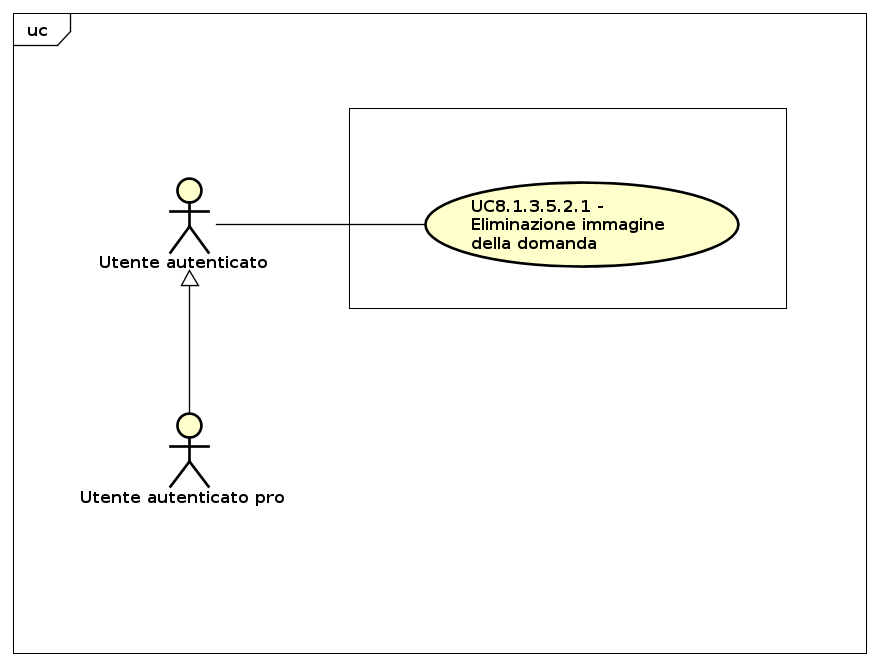
\includegraphics[scale=0.45,keepaspectratio]{UML/UC8_1_3_5_2.png}
	\caption{UC8.1.3.5.2: Inserimento immagine per testo domanda}
\end{figure}
\FloatBarrier
\begin{itemize}
	\item\textbf{Attori}: utente autenticato, utente autenticato pro;
	\item\textbf{Descrizione}: l'attore può inserire un'immagine relativa al testo della domanda;
	\item\textbf{Precondizione}: l'attore ha selezionato la funzionalità di creazione della domanda a ordinamento di immagini; 
	\item \textbf{Postcondizione}: l'attore ha inserito un'immagine relativa al testo della domanda;
	\item\textbf{Scenario principale}: 
		\begin{enumerate}
			\item L'attore può eliminare l'immagine inserita (UC8.1.3.5.2.1).
		\end{enumerate}
\end{itemize}

\subsubsection{Caso d'uso UC8.1.3.5.2.1: Eliminazione immagine della domanda}
\begin{itemize}
	\item\textbf{Attori}: utente autenticato, utente autenticato pro;
	\item\textbf{Descrizione}: l'attore può rimuovere l'immagine, relativa al testo della domanda, che era stata inserita precedentemente;
	\item\textbf{Precondizione}: l'attore ha inserito un immagine relativa al testo della domanda;
	\item \textbf{Postcondizione}: l'attore ha eliminato l'immagine relativa alla domanda;
	\item\textbf{Scenario principale}: l'attore rimuove l'immagine relativa alla domanda. 
\end{itemize}

\subsubsection{Caso d'uso UC8.1.3.5.3: Inserimento immagini come risposta}
\label{UC8.1.3.5.3}
\begin{figure}[h]
	\centering
	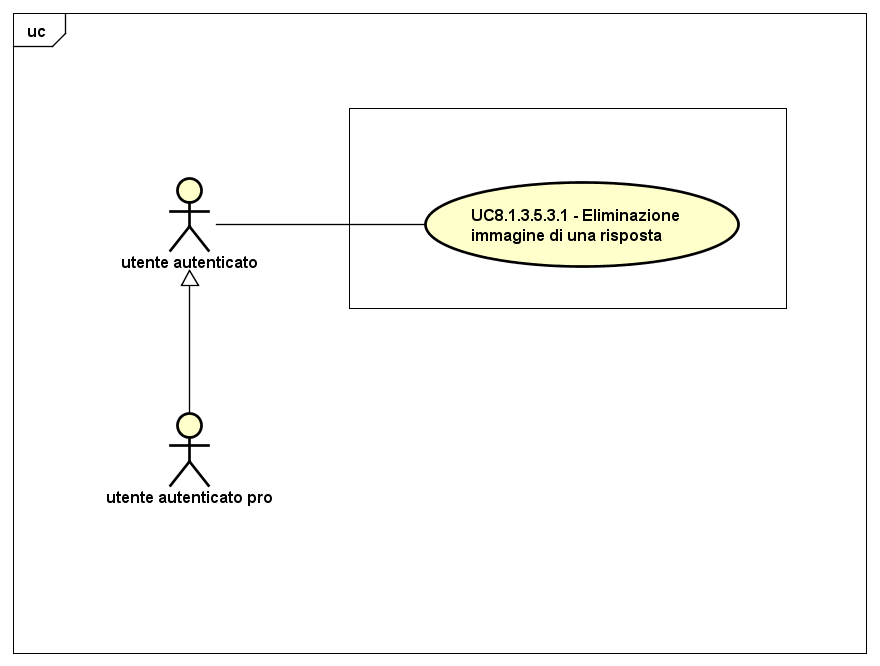
\includegraphics[scale=0.45,keepaspectratio]{UML/UC8_1_3_5_3.png}
	\caption{UC8.1.3.5.3: Inserimento immagini come risposta}
\end{figure}
\begin{itemize}
	\item\textbf{Attori}: utente autenticato, utente autenticato pro;
	\item\textbf{Descrizione}: l'attore può inserire le immagini come risposta alla domanda e indicare la soluzione di questa mettendole nell'ordine corretto;
	\item\textbf{Precondizione}: l'attore ha selezionato la funzionalità di creazione della domanda a ordinamento di immagini; 
	\item \textbf{Postcondizione}: l'attore ha inserito delle immagini come risposta alla domanda e le ha ordinate in base alla soluzione di questa;
	\item\textbf{Scenario principale}:
		\begin{enumerate}
			\item L'attore può eliminare un'immagine inserita (UC8.1.3.5.3.1).
		\end{enumerate}
\end{itemize}
\subsubsection{Caso d'uso UC8.1.3.5.3.1: Eliminazione immagine come risposta}
\begin{itemize}
	\item\textbf{Attori}: utente autenticato, utente autenticato pro;
	\item\textbf{Descrizione}: l'attore può rimuovere un'immagine inserita come risposta;
	\item\textbf{Precondizione}: l'attore ha inserito almeno un'immagine come risposta; 
	\item \textbf{Postcondizione}: l'attore ha eliminato un'immagine relativa alla risposta;
	\item\textbf{Scenario principale}: l'attore rimuove un'immagine relativa alla risposta. 
\end{itemize}
